% This is "sig-alternate.tex" V2.1 April 2013
% This file should be compiled with V2.5 of "sig-alternate.cls" May 2012
%
% This example file demonstrates the use of the 'sig-alternate.cls'
% V2.5 LaTeX2e document class file. It is for those submitting
% articles to ACM Conference Proceedings WHO DO NOT WISH TO
% STRICTLY ADHERE TO THE SIGS (PUBS-BOARD-ENDORSED) STYLE.
% The 'sig-alternate.cls' file will produce a similar-looking,
% albeit, 'tighter' paper resulting in, invariably, fewer pages.
%
% ----------------------------------------------------------------------------------------------------------------
% This .tex file (and associated .cls V2.5) produces:
%       1) The Permission Statement
%       2) The Conference (location) Info information
%       3) The Copyright Line with ACM data
%       4) NO page numbers
%
% as against the acm_proc_article-sp.cls file which
% DOES NOT produce 1) thru' 3) above.
%
% Using 'sig-alternate.cls' you have control, however, from within
% the source .tex file, over both the CopyrightYear
% (defaulted to 200X) and the ACM Copyright Data
% (defaulted to X-XXXXX-XX-X/XX/XX).
% e.g.
% \CopyrightYear{2007} will cause 2007 to appear in the copyright line.
% \crdata{0-12345-67-8/90/12} will cause 0-12345-67-8/90/12 to appear in the copyright line.
%
% ---------------------------------------------------------------------------------------------------------------
% This .tex source is an example which *does* use
% the .bib file (from which the .bbl file % is produced).
% REMEMBER HOWEVER: After having produced the .bbl file,
% and prior to final submission, you *NEED* to 'insert'
% your .bbl file into your source .tex file so as to provide
% ONE 'self-contained' source file.
%
% ================= IF YOU HAVE QUESTIONS =======================
% Questions regarding the SIGS styles, SIGS policies and
% procedures, Conferences etc. should be sent to
% Adrienne Griscti (griscti@acm.org)
%
% Technical questions _only_ to
% Gerald Murray (murray@hq.acm.org)
% ===============================================================
%
% For tracking purposes - this is V2.0 - May 2012

\documentclass{sig-alternate-05-2015}
\usepackage{listings}

\begin{document}

% Copyright
%\setcopyright{acmlicensed}
%\setcopyright{rightsretained}
%\setcopyright{usgov}
%\setcopyright{usgovmixed}
%\setcopyright{cagov}
%\setcopyright{cagovmixed}
%
% --- Author Metadata here ---

%\CopyrightYear{2007} % Allows default copyright year (20XX) to be over-ridden - IF NEED BE.
%\crdata{0-12345-67-8/90/01}  % Allows default copyright data (0-89791-88-6/97/05) to be over-ridden - IF NEED BE.
% --- End of Author Metadata ---

\title{Single Core Design Space Exploration}
\subtitle{ECE 568: Advanced Microprocessor Architecture, Spring 2016}
%
% You need the command \numberofauthors to handle the 'placement
% and alignment' of the authors beneath the title.
%
% For aesthetic reasons, we recommend 'three authors at a time'
% i.e. three 'name/affiliation blocks' be placed beneath the title.
%
% NOTE: You are NOT restricted in how many 'rows' of
% "name/affiliations" may appear. We just ask that you restrict
% the number of 'columns' to three.
%
% Because of the available 'opening page real-estate'
% we ask you to refrain from putting more than six authors
% (two rows with three columns) beneath the article title.
% More than six makes the first-page appear very cluttered indeed.
%
% Use the \alignauthor commands to handle the names
% and affiliations for an 'aesthetic maximum' of six authors.
% Add names, affiliations, addresses for
% the seventh etc. author(s) as the argument for the
% \additionalauthors command.
% These 'additional authors' will be output/set for you
% without further effort on your part as the last section in
% the body of your article BEFORE References or any Appendices.

\numberofauthors{1} %  in this sample file, there are a *total*
% of EIGHT authors. SIX appear on the 'first-page' (for formatting
% reasons) and the remaining two appear in the \additionalauthors section.
%
\author{
% You can go ahead and credit any number of authors here,
% e.g. one 'row of three' or two rows (consisting of one row of three
% and a second row of one, two or three).
%
% The command \alignauthor (no curly braces needed) should
% precede each author name, affiliation/snail-mail address and
% e-mail address. Additionally, tag each line of
% affiliation/address with \affaddr, and tag the
% e-mail address with \email.
%
% 1st. author
\alignauthor
Anthony Gallotta
       \email{agallo4@uic.edu}
}
% There's nothing stopping you putting the seventh, eighth, etc.
% author on the opening page (as the 'third row') but we ask,
% for aesthetic reasons that you place these 'additional authors'
% in the \additional authors block, viz.
\date{05 March 2016}
% Just remember to make sure that the TOTAL number of authors
% is the number that will appear on the first page PLUS the
% number that will appear in the \additionalauthors section.

\maketitle
\begin{abstract}
This paper seeks to find the best single core superscalar architecture for a given benchmark application by experimenting with different architectures for branch prediction, memory systems, functional units, data path, and other areas. The metrics used to define the "best" architecture are \textit{performance} as instructions per cycle (IPC) and \textit{performance-energy} as the energy delay product (EDP).
\end{abstract}


%
% The code below should be generated by the tool at
% http://dl.acm.org/ccs.cfm
% Please copy and paste the code instead of the example below. 
%
%\begin{CCSXML}
%<ccs2012>
% <concept>
%  <concept_id>10010520.10010553.10010562</concept_id>
%  <concept_desc>Computer systems organization~Embedded systems</concept_desc>
%  <concept_significance>500</concept_significance>
% </concept>
% <concept>
%  <concept_id>10010520.10010575.10010755</concept_id>
%  <concept_desc>Computer systems organization~Redundancy</concept_desc>
%  <concept_significance>300</concept_significance>
% </concept>
% <concept>
%  <concept_id>10010520.10010553.10010554</concept_id>
%  <concept_desc>Computer systems organization~Robotics</concept_desc>
%  <concept_significance>100</concept_significance>
% </concept>
% <concept>
%  <concept_id>10003033.10003083.10003095</concept_id>
%  <concept_desc>Networks~Network reliability</concept_desc>
%  <concept_significance>100</concept_significance>
% </concept>
%</ccs2012>  
%\end{CCSXML}

%\ccsdesc[500]{Computer systems organization~Embedded systems}
%\ccsdesc[300]{Computer systems organization~Redundancy}
%\ccsdesc{Computer systems organization~Robotics}
%\ccsdesc[100]{Networks~Network reliability}


%
% End generated code
%

%
%  Use this command to print the description
%
\printccsdesc

% We no longer use \terms command
%\terms{Theory}

%\keywords{ACM proceedings; \LaTeX; text tagging}

\section{Introduction}
This study evaluates a single core superscalar architecture using the SimpleScalar simulator suite, seeking the best configuration for the \texttt{eeg} benchmark application. A base architecture was given, and design modifications were then made in four groups, branch prediction, memory system, functional units, and data path. In the first phase of design space exploration, tuning one parameter at a time. In the second stage, closely related parameters within the same groups are tuned together. Finally, the best configurations across groups are combined to formulate the best found architecture. For each configuration we observe performance (IPC) and performance-energy (EDP), calculated as $ (CPI * energy/cycle) * CPI $. The "best" configuration seeks to maximize performance, and minimize performance-energy.

\section{Simulation}
Simulations of the \texttt{eeg} application benchmark were performed using \texttt{sim-outorder}. The base configuration had performance of 1.5226 IPC, and a performance-energy product of 219.68. While many parameter changes were tested, unless otherwise noted, all graphs that follow show only configurations that outperformed the base configuration in at least one of these metrics\footnote{\label{note1}Results from all configurations, along with the configuration files themselves and scripts used in this simulation are available at \url{https://github.com/tonygallotta/ece568-single-core-dse.git}}. The most desirable configurations will lie in the lower right side of the graphs that follow.

To gain some direction in performance tuning, the instruction profile for the benchmark was first evaluated using \texttt{sim-profile}. As shown in table \ref{table:instr_profile}, the benchmark is primarily an integer program. Given this instruction breakdown, most of the performance tuning was focused on branch prediction and the memory system. For each group, the initial focus was on one attribute at a time. Once good parameters to tune were found, some combinations of parameters within each group were attempted as well to further improve performance.

Simulations were executed by providing configuration files to sim-outorder. A sample configuration file and output are provided at the end of this report. Simulation results were then processed by a series of \texttt{bash} scripts to generate a CSV file of the results, which was processed using Python and the \texttt{matplotlib} library to generate the figures in this report\footnote{See footnote 1}.

\begin{table}
\centering
\caption{Instruction Profile for \texttt{eeg}}
\label{table:instr_profile}
\begin{tabular}{| c | c | l | } \hline
Type & Count & Percent \\ \hline
load             & 171,182,879 & 20.30 \\ \hline
store            &  84,069,724 &  9.97 \\ \hline
uncond branch    &  60,740,822 &  7.20 \\ \hline
cond branch      &  59,922,458 &  7.11 \\ \hline
int computation  & 335,861,146 & 39.84 \\ \hline
fp computation   & 131,306,086 & 15.57 \\ \hline
trap             &      1,035 &  0.00 \\
\hline\end{tabular}
\end{table}

\subsection{Branch Prediction}
%btb-128-2 wins.
The first branch prediction change attempted was to use static prediction. This strategy resulted in much worse performance by both metrics and was quickly abandoned. Next, some tuning was made with the default bimodal branch predictor, which uses a simple strategy of picking the most common direction. Sticking with this scheme, the branch target buffer (BTB) size and associativity was adjusted. In figure \ref{graph:bp_results}, the points labeled as \texttt{bp-btb-<sets>-<associativity>} indicate the results of these adjustments. The BTB configuration of 128 sets with 2 way associativity is able to achieve the same performance as the base configuration, with a much lower EDP. 

Two level branch predictors use a combination of the last $k$ historical  branch outcomes, as well as the behavior for a specific pattern of previous branches \cite{yeh1993comparison}. While many of the 2 level configurations did not perform the base configuration, the 2 level Global Address (GA) branch predictor with a 4 wide history (bp-2level-hist-4) did achieve a better IPC. Combining these configuration changes (bp-comb-128-2) by keeping the best found BTB size and using a combined bimodal and 2-level branch predictor gives about a 5\% performance-energy improvement over the base configuration.

A perfect branch prediction scheme is plotted for comparison. Suprisingly, the perfect branch predictor achieves a lower IPC than many of the experimental configurations. The simulator documentation does not describe in detail how the perfect branch predictor operates, so it may be that they are modeling a higher latency for the perfect predictor.

\begin{figure}
\centering
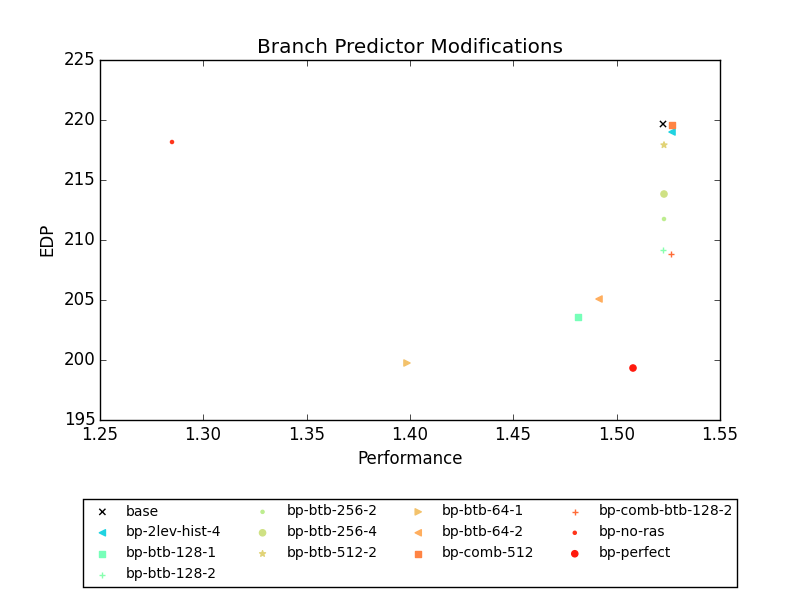
\includegraphics[scale=0.4]{./bp}
\caption{Branch Predictor Variation results}
\label{graph:bp_results}
\end{figure}

\subsection{Memory System}
The simulator has a 2 level cache hierarchy, and different sizes, associativity, block sizes, and replacement policies were experimented with at each level, and for both instruction and data caches. Cache parameter modifications were not chosen to align with the program in any way, they were simply chosen to cast a wide net over the design space and see which modifications may show promise. For example, most parameters were increased and decreased by a power of 2 for an initial experiment. If that modification resulted in a performance improvement, another power of 2 increase or decrease was attempted, until performance started to degrade.

\subsubsection{L1 Cache}
As figure \ref{graphdl1all} shows, increasing the size of the L1 data cache (sets) did not result in significant IPC improvements relative to their increased power consumption. Increasing the block size to 64 while keeping the total L1 size the same (bsize-64) yields the best result in terms of both of our architecture goals.

Figure \ref{graphil1all} shows similar results for the instruction cache - a block size of 64 performs best.

\subsubsection{L2 Cache}
At the L2 cache, we see once again from figures \ref{graph:memdl2separated}, \ref{graph:memil2separated}, and \ref{graph:meml2unified} that a unified cache with a decreased block size performs best.

\begin{figure}
\centering
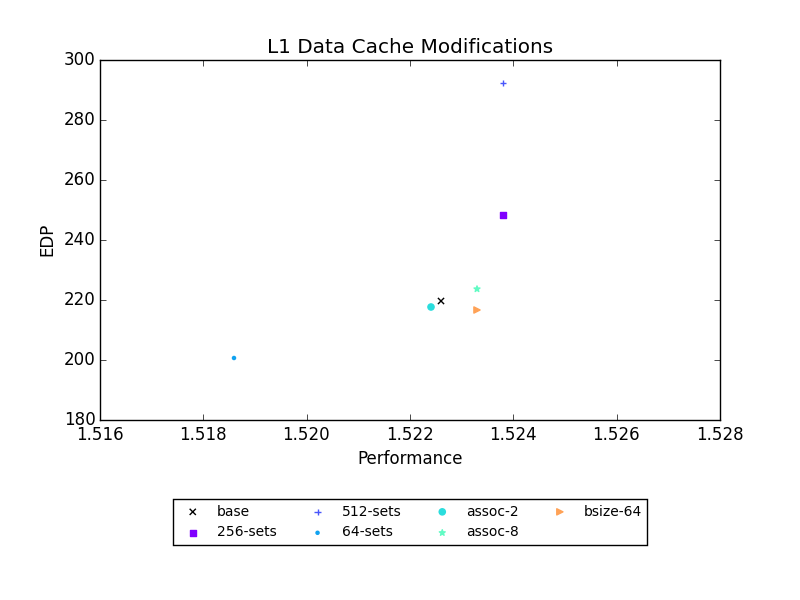
\includegraphics[scale=0.4]{../mem-dl1-all}
\caption{Modifications for L1 data cache}
\label{graphdl1all}
\end{figure}


\begin{figure}
\centering
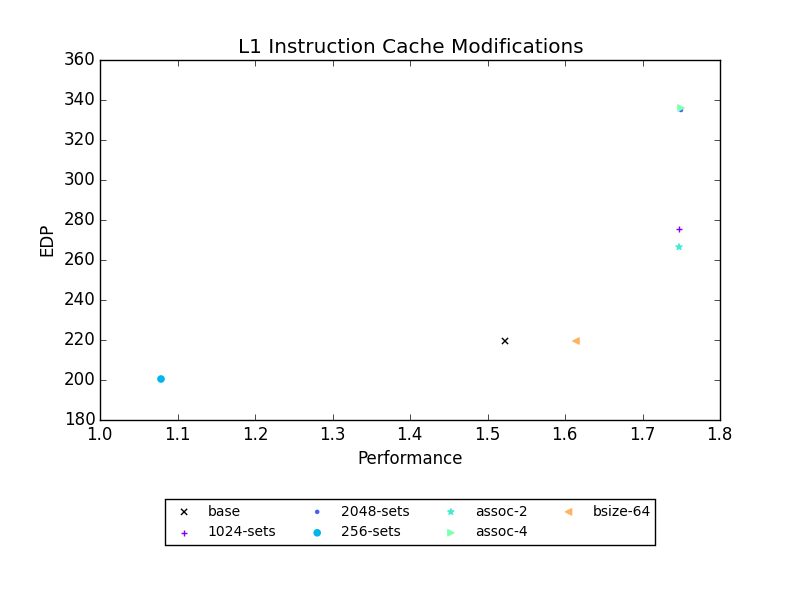
\includegraphics[scale=0.4]{../mem-il1}
\caption{Modifications for L1 instruction cache}
\label{graphil1all}
\end{figure}

\begin{figure}
\centering
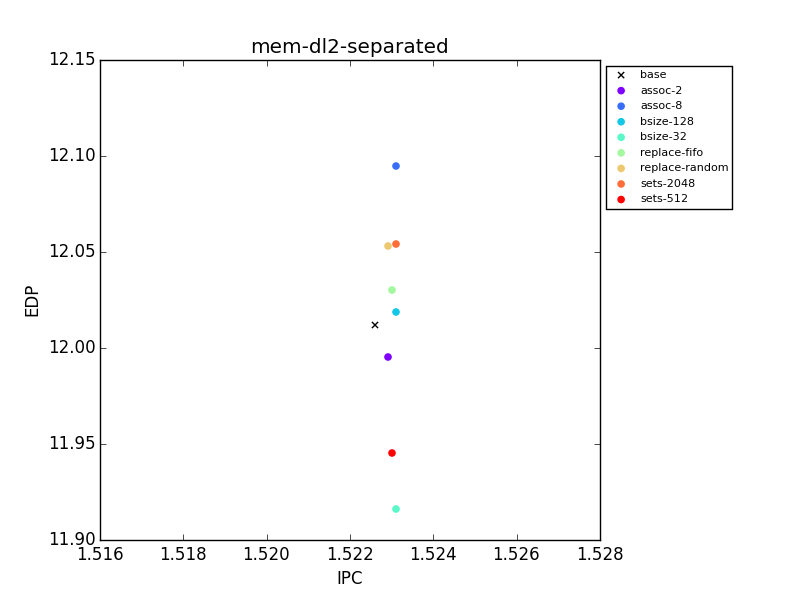
\includegraphics[scale=0.4]{../mem-dl2-separated}
\caption{Modifications for L2 data cache}
\label{graph:memdl2separated}
\end{figure}

\begin{figure}
\centering
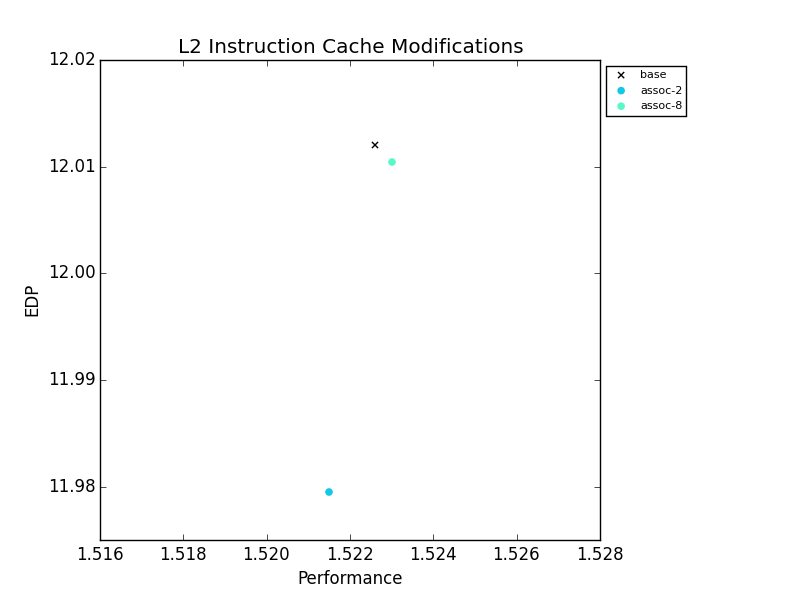
\includegraphics[scale=0.4]{../mem-il2-separated}
\caption{Modifications for L2 instruction cache}
\label{graph:memil2separated}
\end{figure}

\begin{figure}
\centering
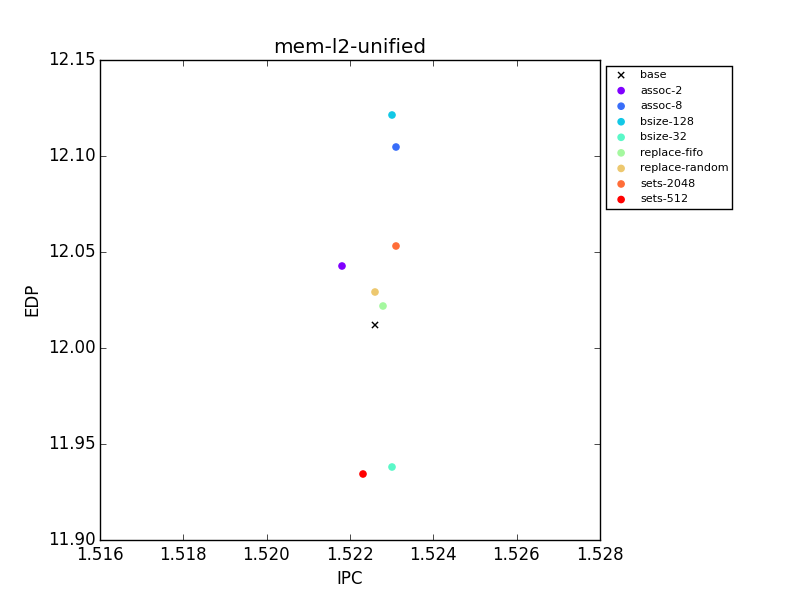
\includegraphics[scale=0.4]{../mem-l2-unified}
\caption{Unified L2 cache}
\label{graph:meml2unified}
\end{figure}

\subsection{Functional Units}
Since this program is integer focused, one of the first modifications made to increase performance-energy was to decrease the number of floating point units. As figure \ref{graph:func} shows (fpalu-2), the number of floating point ALUs can be decreased from 4 to 2 with no change in IPC. Interestingly, increasing the number of FP multipliers does increase IPC, at a slight cost to EDP.

The integer functional units seem to already be at a sweet spot. Increasing the number of integer ALUs or multipliers does not result in significant IPC gains. The base configuration only has 1 integer multiplier, so this cannot be decreased, but decreasing the number of ALUs results in significant IPC losses.

\begin{figure}
\centering
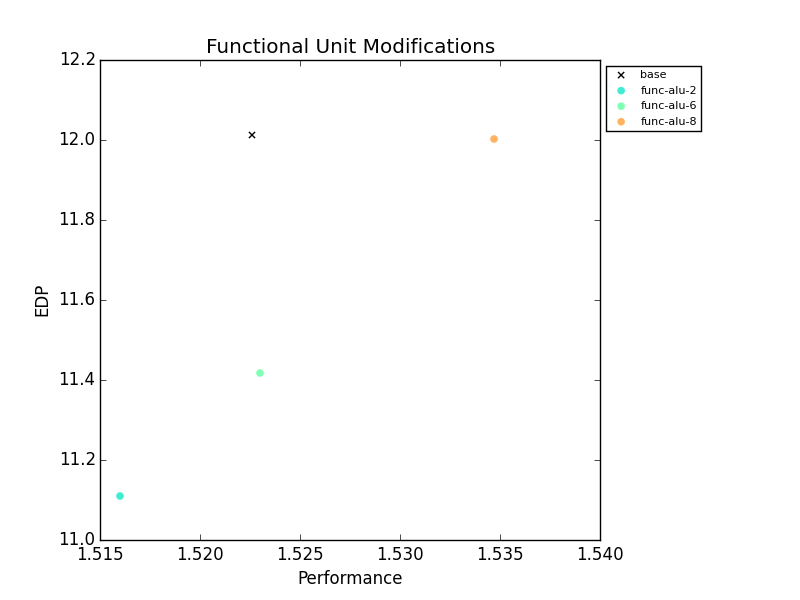
\includegraphics[scale=0.4]{../func}
\caption{Functional unit modifications}
\label{graph:func}
\end{figure}

\subsection{Data Path}
The data path attributes modified were in-order vs. out of order (base) issue, instruction decode and issue width, and size of the reorder. On their own, none of these modifications result in a good trade off of performance vs. EDP. Even when tuning closely related parameters together, such as instruction decode and issue width, there are no clear performance improvements. These attributes will be revisited when tuning parameters are combined since other modifications may make a wider instruction issue or reorder buffer more useful. 

\begin{figure}
\centering
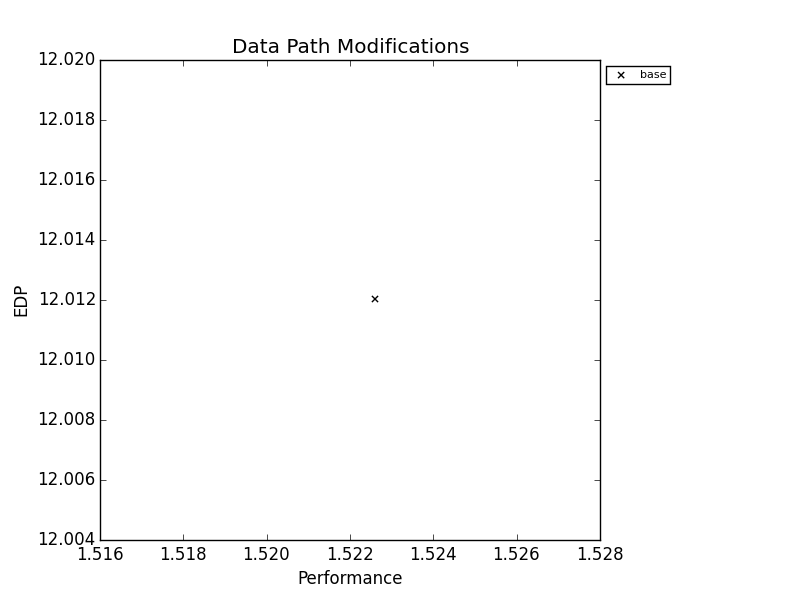
\includegraphics[scale=0.4]{../dp}
\caption{Data path modifications}
\label{graph:meml2unified}
\end{figure}


\section{Cross Group Simulations}
For the final group of simulations, the best parameter modifications from each group were selected, and combined. The only exception was between the L1 and L2 caches. While a block size of 64 performed best for the L1 cache, the best performance for the L2 cache was observed under a block size of 32. In practice, this doesn't really make sense since the L1 cache is typically a subest of the L2 cache, and the L1 cache would have to load 2 blocks to fill 1 of its own. sim-outorder did not even allow this configuration, and crashed when attempting to use a smaller block size in the L2 cache than L1. Therefore, the block size was kept consistent between the 2 levels, and both 32 (combined-blocksize-32) and 64 (combined-base) were tried for the combined configuration. As seen in figure \ref{graph:combined}, the block size of 64 achieved a pretty large increase in IPC without a large EDP sacrifice, so this architecture was chosen to proceed with.

In this step, modifications to the instruction issue width were revisited, tuning all related parameters together (fetch, decode, issue, and commit width), however the results were fairly extreme. An issue width of 8 resulted in a 16\% IPC increase, but also increased the EDP by 3\%. Dropping the width down to 2 resulted in a significant EDP decrease (25\%), but also dropped IPC by 20\%. The architecture that achieved the best performance overall was INSERT_HERE, achieving roughly a 15\% decrease in performance-energy, and 7\% improvement in performance.
\begin{figure}
\centering
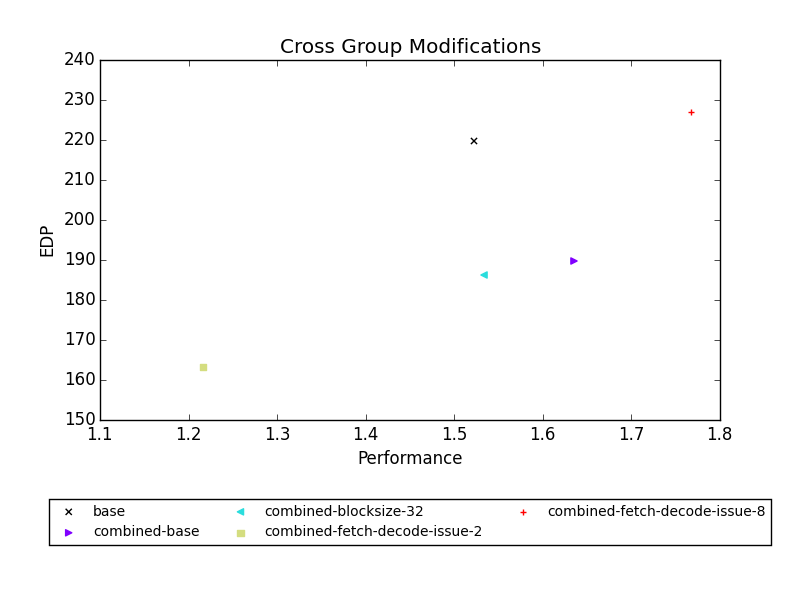
\includegraphics[scale=0.4]{../combined}
\caption{Cross group modifications}
\label{graph:combined}
\end{figure}

\section{Conclusions}
Simulation tools can be useful in tuning architectures for good performance for a specific application. Observing the instruction profile for a given application can be helpful in making educated guesses when tuning architecture details, but some parameters like memory configurations can be difficult to estimate, and can be easier to tune by testing a wide range of parameters and observing their effects.

\newpage
\onecolumn
\appendix

\section{Results of all simulations}

\begin{table}
\centering
\label{table:all_results}
\begin{tabular}{| c | c | c | l | } \hline
Category & Config & IPC & EDP \\ \hline
base & base & 1.5226 & 219.68 \\ \hline
bp & bp-2lev-GAg & 1.4142 & 223.2 \\ \hline
bp & bp-2lev-GAp & 1.4288 & 222.5 \\ \hline
bp & bp-2lev-PAg-l1-16 & 1.5143 & 220.96 \\ \hline
bp & bp-2lev-PAg-l1-2 & 1.4255 & 221.83 \\ \hline
bp & bp-2lev-PAp-l1-2 & 1.5184 & 220.17 \\ \hline
bp & bp-2lev-PAp-l1-4 & 1.5320 & 221.83 \\ \hline
bp & bp-2lev-gshare & 1.5259 & 220.15 \\ \hline
bp & bp-2lev-hist-16 & 1.4142 & 223.8 \\ \hline
bp & bp-2lev-hist-4 & 1.5266 & 218.98 \\ \hline
bp & bp-2lev-l1-128 & 1.5378 & 218.41 \\ \hline
bp & bp-2lev-l1-64 & 1.5380 & 219.7 \\ \hline
bp & bp-2lev-l1-8 & 1.4287 & 220.19 \\ \hline
bp & bp-2lev-l2-512 & 1.4108 & 223.55 \\ \hline
bp & bp-2lev-xor & 1.5235 & 220.29 \\ \hline
bp & bp-2lev & 1.4288 & 221.57 \\ \hline
bp & bp-btb-1024-2 & 1.5230 & 219.7 \\ \hline
bp & bp-btb-1024-4 & 1.5230 & 225.08 \\ \hline
bp & bp-btb-128-1 & 1.4811 & 203.62 \\ \hline
bp & bp-btb-128-2 & 1.5224 & 209.2 \\ \hline
bp & bp-btb-256-2 & 1.5228 & 211.77 \\ \hline
bp & bp-btb-256-4 & 1.5230 & 213.86 \\ \hline
bp & bp-btb-512-2 & 1.5229 & 217.93 \\ \hline
bp & bp-btb-64-1 & 1.3987 & 199.74 \\ \hline
bp & bp-btb-64-2 & 1.4914 & 205.07 \\ \hline
bp & bp-comb-2048 & 1.5270 & 220.73 \\ \hline
bp & bp-comb-512 & 1.5269 & 219.54 \\ \hline
bp & bp-comb-btb-128-2 & 1.5263 & 208.81 \\ \hline
bp & bp-comb & 1.5270 & 219.93 \\ \hline
bp & bp-no-ras & 1.2846 & 218.17 \\ \hline
bp & bp-nottaken & 0.7513 & 272.76 \\ \hline
bp & bp-perfect & 1.5078 & 199.34 \\ \hline
bp & bp-ras-16 & 1.5231 & 220.8 \\ \hline
bp & bp-taken & 0.7578 & 281.58 \\ \hline
combined & 2lev-hist-4 & 1.6352 & 187.72 \\ \hline
combined & base & 1.6352 & 189.72 \\ \hline
combined & blocksize-32 & 1.5339 & 186.33 \\ \hline
combined & fetch-decode-issue-2 & 1.2162 & 163.13 \\ \hline
combined & fetch-deodec-issue-8 & 1.7670 & 226.91 \\ \hline
combined & fpmul-1 & 1.6152 & 187.55 \\ \hline
\end{tabular}
\end{table}

\begin{table}
\centering
\label{table:all_results_2}
\begin{tabular}{| c | c | c | l | } \hline
Category & Configuration & IPC & EDP \\ \hline
dp & dp-decode-2 & 1.2894 & 228.32 \\ \hline
dp & dp-decode-8 & 1.5230 & 221.16 \\ \hline
dp & dp-decode-issue-8 & 1.5323 & 298.64 \\ \hline
dp & dp-inorder & 0.8050 & 210.34 \\ \hline
dp & dp-issue-2 & 1.2087 & 180.59 \\ \hline
dp & dp-issue-8 & 1.5323 & 298.45 \\ \hline
dp & dp-ruu-8 & 1.2721 & 201.05 \\ \hline
func & func-alu-2 & 1.4094 & 209.63 \\ \hline
func & func-alu-6 & 1.5230 & 229.5 \\ \hline
func & func-alu-8 & 1.5230 & 239.39 \\ \hline
func & func-fpalu-1 & 1.5160 & 187.15 \\ \hline
func & func-fpalu-2 & 1.5230 & 198.54 \\ \hline
func & func-fpmul-2 & 1.5347 & 221.12 \\ \hline
func & func-imul-2 & 1.5230 & 221.43 \\ \hline
func & func-imul-3 & 1.5230 & 219.94 \\ \hline
mem & mem-dl1-128-64-2 & 1.5227 & 215.25 \\ \hline
mem & mem-dl1-256-sets & 1.5238 & 248.48 \\ \hline
mem & mem-dl1-64-sets & 1.5186 & 200.63 \\ \hline
mem & mem-dl1-assoc-2 & 1.5224 & 217.52 \\ \hline
mem & mem-dl1-assoc-8 & 1.5233 & 223.67 \\ \hline
mem & mem-dl1-bsize-128 & 0.1143 & 529.49 \\ \hline
mem & mem-dl1-bsize-16 & 1.5223 & 223.46 \\ \hline
mem & mem-dl1-bsize-64 & 1.5233 & 216.74 \\ \hline
mem & mem-dl1-replace-fifo & 1.5225 & 221.42 \\ \hline
mem & mem-dl1-replace-random & 1.5217 & 219.78 \\ \hline
mem & mem-dl2-assoc-2 & 1.5218 & 220.7 \\ \hline
mem & mem-dl2-assoc-8 & 1.5231 & 223.16 \\ \hline
mem & mem-dl2-bsize-128 & 1.5230 & 223.76 \\ \hline
mem & mem-dl2-bsize-32 & 1.5230 & 217.05 \\ \hline
mem & mem-dl2-replace-fifo & 1.5228 & 220.07 \\ \hline
mem & mem-dl2-replace-random & 1.5226 & 220.31 \\ \hline
mem & mem-dl2-separated-assoc-2 & 1.5229 & 219.15 \\ \hline
mem & mem-dl2-separated-assoc-8 & 1.5231 & 222.78 \\ \hline
mem & mem-dl2-separated-bsize-128 & 1.5231 & 219.99 \\ \hline
mem & mem-dl2-separated-bsize-32 & 1.5231 & 216.26 \\ \hline
mem & mem-dl2-separated-replace-fifo & 1.5230 & 220.42 \\ \hline
mem & mem-dl2-separated-replace-random & 1.5229 & 221.26 \\ \hline
mem & mem-dl2-separated-sets-2048 & 1.5231 & 221.29 \\ \hline
mem & mem-dl2-separated-sets-512 & 1.5230 & 217.32 \\ \hline
mem & mem-dl2-sets-2048 & 1.5231 & 221.27 \\ \hline
mem & mem-dl2-sets-512 & 1.5223 & 216.82 \\ \hline
mem & mem-il1-1024-sets & 1.7466 & 275.48 \\ \hline
mem & mem-il1-256-sets & 1.0784 & 200.54 \\ \hline
mem & mem-il1-assoc-2 & 1.7473 & 266.75 \\ \hline
mem & mem-il1-assoc-4 & 1.7495 & 336.25 \\ \hline
mem & mem-il1-bsize-16 & 1.4704 & 239.86 \\ \hline
mem & mem-il1-bsize-64 & 1.6141 & 219.35 \\ \hline
mem & mem-il1-fifo & 1.5217 & 220.14 \\ \hline
mem & mem-il1-random & 1.5217 & 219.74 \\ \hline
mem & mem-il2-separated-assoc-2 & 1.5231 & 220.62 \\ \hline
mem & mem-il2-separated-assoc-8 & 1.5231 & 220.0 \\ \hline
mem & mem-il2-separated-bsize-128 & 1.5215 & 218.33 \\ \hline
mem & mem-il2-separated-bsize-32 & 1.5230 & 219.69 \\ \hline
mem & mem-il2-separated-replace-fifo & 1.5231 & 219.93 \\ \hline
mem & mem-il2-separated-replace-random & 1.5231 & 221.27 \\ \hline
mem & mem-il2-separated-sets-2048 & 1.5231 & 219.85 \\ \hline
mem & mem-il2-separated-sets-512 & 1.5231 & 220.71 \\ \hline
\end{tabular}
\end{table}

\newpage
\section{Configuration for best found architecture (comb-2lev-hist-4)}
\lstinputlisting{../configs/step3/combined-2lev-hist-4.cfg}

\section{Simulation output for best found architecture (comb-2lev-hist-4)}
\lstinputlisting{../results/combined-2lev-hist-4.out}

%
% The following two commands are all you need in the
% initial runs of your .tex file to
% produce the bibliography for the citations in your paper.
\bibliographystyle{abbrv}
\bibliography{sigproc}  % sigproc.bib is the name of the Bibliography in this case
% You must have a proper ".bib" file
%  and remember to run:
% latex bibtex latex latex
% to resolve all references

\end{document}
